\chapter{Mathematical Foundations, from First Principles}
\label{ch:math}

\epigraph{Mathematics is the art of giving the same name to different
things.}{Henri Poincar\'e}

The arguments of this thesis---that three protocols compose into one substrate,
that conformance is three-valued, that convergence is a phase transition, that a
repository can be read as a curved space of trajectories---are stated informally
in \cref{ch:framework} and instantiated in \cref{ch:artifact}. This chapter
supplies their mathematics, and it does so \emph{from first principles}: each
construct is built from sets and axioms, with definitions, and with proofs of the
propositions the later chapters invoke. The intent is that no subsequent claim
rests on borrowed authority; where the thesis says ``composition'', ``lattice'',
``latent heat'', or ``curvature'', this chapter says exactly what is meant.

We make no claim to new mathematics. The contribution is the \emph{derivation of
the thesis's own constructs} within standard mathematics, so that they are
falsifiable rather than merely evocative. Five pillars are built, and a short
synthesis (\cref{sec:synthesis-functor}) draws them into a single functor; each
terminates in a result used later:

\begin{description}[leftmargin=1.6em,style=nextline]
  \item[Pillar I --- The algebra of composition (\cref{sec:alg}).] From monoids
  through categories, functors, adjunctions, monoidal categories, and operads to
  the \emph{Decoupling Theorem} (\cref{thm:decoupling}), which is the algebraic
  engine behind the phase transition's mechanism (\cref{prop:discontinuous}).
  \item[Pillar II --- The order-theoretic logic of conformance.] From posets and
  lattices to Kleene's and Belnap's many-valued logics, formalising the
  \code{ConformanceVector} (\cref{lst:cv}) and \cref{prin:three-valued}.
  \item[Pillar III --- The analysis of phase transitions.] From limits and
  continuity to Landau's free-energy expansion and a from-scratch derivation of
  the Clausius--Clapeyron relation and the latent heat that anchors
  \cref{sec:fw-latent}.
  \item[Pillar IV --- The geometry of law-state.] From topological spaces through
  smooth manifolds, connections, and curvature to gradient flow, formalising the
  manifold metaphors of \code{AGENTS.md} (repository as manifold, failsets as
  curvature, admissibility as $\Phi_G = 0$).
  \item[Pillar V --- Measure, probability, and information.] From $\sigma$-algebras
  through entropy and Fisher information, making ``receipts are proof measure'' a
  literal measure, recasting non-collapse as a data-processing inequality, and
  identifying the manifold of Pillar~IV with a statistical manifold via the
  Fisher--Rao metric.
\end{description}

A reader fluent in these areas may treat the chapter as fixing notation and skip
to \cref{ch:framework}; a reader who wants the thesis to stand on its own will
find here the load it is asked to bear. Pillars are developed in the order above;
forward references to later chapters are deliberate, marking where each piece of
mathematics is spent.

\section{Pillar I --- The Algebra of Composition}
\label{sec:alg}

The thesis's central structural claim is about \emph{composition}: that a
capability isolated behind a contract can be recombined freely, turning an
$M\times N$ burden into $M+N$ (\cref{tab:three-decouplings}). Composition is the
subject matter of algebra and, at its most general, of category theory. We build
the needed apparatus from sets.

\subsection{Sets, maps, and the combinatorics of integration}
\label{sec:alg-sets}

We take as primitive the notions of \emph{set}, \emph{element} ($x\in X$), and
\emph{function} $f\colon X\to Y$ assigning to each $x\in X$ a unique
$f(x)\in Y$. For finite $X$ write $|X|$ for its cardinality. The
\emph{product} $X\times Y=\{(x,y):x\in X,\ y\in Y\}$ satisfies
$|X\times Y|=|X|\,|Y|$. These suffice to state the problem every protocol in this
thesis attacks.

\begin{definition}[Integration problem]
\label{def:integration}
Let $E$ be a set of \emph{clients} (editors, hosts, agents) and $L$ a set of
\emph{providers} (language servers, tools, agents). A \emph{bespoke integration}
is a partial function assigning to a pair $(e,\ell)\in E\times L$ a connector
realising the capability of $\ell$ in $e$. Full coverage requires a connector for
every pair.
\end{definition}

\begin{lemma}[Quadratic cost of bespoke integration]
\label{lem:mn}
Full bespoke coverage of \cref{def:integration} requires $|E|\,|L|$ connectors.
\end{lemma}
\begin{proof}
Full coverage demands a connector for each $(e,\ell)\in E\times L$; distinct
pairs need distinct connectors because each names a distinct client--provider
interface. Hence the count equals $|E\times L| = |E|\,|L|$.
\end{proof}

\begin{construction}[Hub interposition]
\label{con:hub}
Introduce a single object $H$ (a \emph{protocol}) and replace each pair-connector
by two contract-conformances: a client side $e\rightsquigarrow H$ for each $e\in
E$, and a provider side $H\rightsquigarrow \ell$ for each $\ell\in L$. A pair
$(e,\ell)$ is served by routing $e\rightsquigarrow H\rightsquigarrow \ell$.
\end{construction}

\begin{proposition}[Linear cost via a hub]
\label{prop:mplusn}
\Cref{con:hub} achieves full coverage with $|E|+|L|$ contract-conformances, and
$|E|+|L| \le |E|\,|L|$ whenever $|E|,|L|\ge 2$, with the gap
$|E|\,|L|-(|E|+|L|)$ growing without bound.
\end{proposition}
\begin{proof}
Each client and each provider is connected once to $H$, giving $|E|+|L|$
conformances; routing through $H$ serves every pair, so coverage is full. For the
inequality, $|E|\,|L|-|E|-|L|=(|E|-1)(|L|-1)-1\ge 0$ for $|E|,|L|\ge 2$, and
$(|E|-1)(|L|-1)\to\infty$ as either grows.
\end{proof}

\Cref{prop:mplusn} is LSP's founding insight made arithmetic
\citep{lsp-official,lsp-mxn-fcc}. The remainder of the pillar promotes this
arithmetic to structure, so that it can be \emph{composed across strata}---which
is what distinguishes the thesis's fusion claim from a single application of
\cref{prop:mplusn}.

\subsection{Monoids and the free monoid: language as algebra}
\label{sec:alg-monoid}

The objects this thesis calls ``language'' are, at bottom, sequences of symbols
with a notion of concatenation. That is a monoid.

\begin{definition}[Magma, semigroup, monoid]
A \emph{magma} is a set $M$ with a binary operation $\cdot\colon M\times M\to M$.
It is a \emph{semigroup} if $\cdot$ is associative, $a\cdot(b\cdot c)=(a\cdot
b)\cdot c$, and a \emph{monoid} if additionally there is a unit $e$ with $e\cdot
a=a\cdot e=a$. A monoid homomorphism $\varphi\colon (M,\cdot,e)\to(M',\ast,e')$
satisfies $\varphi(a\cdot b)=\varphi(a)\ast\varphi(b)$ and $\varphi(e)=e'$.
\end{definition}

\begin{definition}[Free monoid / Kleene star]
For a set $\Sigma$ (an \emph{alphabet}), the \emph{free monoid} $\Sigma^{*}$ is
the set of finite sequences (\emph{words}) over $\Sigma$, with operation
concatenation and unit the empty word $\varepsilon$. A \emph{formal language} is
a subset $L\subseteq\Sigma^{*}$, and a \emph{trace} is an element of
$\Sigma^{*}$.
\end{definition}

\begin{theorem}[Universal property of the free monoid]
\label{thm:freemon}
For every set $\Sigma$, every monoid $M$, and every function $f\colon\Sigma\to M$,
there is a unique monoid homomorphism $\bar f\colon\Sigma^{*}\to M$ with $\bar
f(a)=f(a)$ for all $a\in\Sigma$.
\end{theorem}
\begin{proof}
Define $\bar f(\varepsilon)=e_M$ and $\bar f(a_1a_2\cdots a_n)=f(a_1)\cdot
f(a_2)\cdots f(a_n)$. This is well defined (words have unique symbol
decompositions), is a homomorphism by associativity of $M$, and restricts to $f$
on $\Sigma$. Any homomorphism agreeing with $f$ on $\Sigma$ must agree on all
words, since it preserves concatenation and unit; hence $\bar f$ is unique.
\end{proof}

\Cref{thm:freemon} is the algebraic content of \cref{def:eventlog}: a
\emph{semantics} for a language $L$ is exactly a monoid (or richer algebra)
homomorphism out of $\Sigma^{*}$, and the ``event-log abstraction'' records the
generating events $\Sigma$ together with the homomorphism that interprets their
compositions. Process mining's \emph{trace} is a free-monoid element; an event
log is a multiset of such elements.

\subsection{Categories}
\label{sec:alg-cat}

Monoids compose elements; categories compose \emph{morphisms} between objects,
and so model client--provider conformance directly.

\begin{definition}[Category]
\label{def:category}
A \emph{category} $\mathcal C$ consists of a class of \emph{objects}
$\operatorname{ob}\mathcal C$; for each ordered pair $(X,Y)$ a set
$\mathcal C(X,Y)$ of \emph{morphisms}; a composition
$\circ\colon\mathcal C(Y,Z)\times\mathcal C(X,Y)\to\mathcal C(X,Z)$; and for each
$X$ an identity $\mathrm{id}_X\in\mathcal C(X,X)$, such that composition is
associative and $\mathrm{id}$ is a two-sided unit:
$h\circ(g\circ f)=(h\circ g)\circ f$ and $\mathrm{id}_Y\circ f=f=f\circ
\mathrm{id}_X$.
\end{definition}

\begin{example}
$\mathbf{Set}$ has sets as objects and functions as morphisms. $\mathbf{Mon}$ has
monoids as objects and homomorphisms as morphisms. A monoid is precisely a
category with one object (its elements are the endomorphisms of that object). A
preorder $(P,\le)$ is a category with at most one morphism $x\to y$, present iff
$x\le y$; associativity and identities are transitivity and reflexivity.
\end{example}

The last example matters: \cref{sec:order} (Pillar~II) treats the conformance
verdict lattice as such a category, so order and composition are the same theory
viewed twice. We model each protocol stratum of \cref{ch:fusion} as a category
$\mathcal P$ whose objects are participants and whose morphisms are admissible
conformances; capability negotiation is the assertion that a morphism exists.

\subsection{Functors, adjunctions, and the decoupling}
\label{sec:alg-functor}

\begin{definition}[Functor]
A \emph{functor} $F\colon\mathcal C\to\mathcal D$ assigns to each object $X$ an
object $FX$ and to each morphism $f\colon X\to Y$ a morphism $Ff\colon FX\to FY$,
preserving identities and composition: $F\,\mathrm{id}_X=\mathrm{id}_{FX}$ and
$F(g\circ f)=Fg\circ Ff$.
\end{definition}

\begin{definition}[Natural transformation]
For functors $F,G\colon\mathcal C\to\mathcal D$, a \emph{natural transformation}
$\eta\colon F\Rightarrow G$ assigns to each $X$ a morphism $\eta_X\colon FX\to GX$
such that for every $f\colon X\to Y$ the square commutes,
$G f\circ\eta_X=\eta_Y\circ F f$:
\[
\begin{tikzcd}[ampersand replacement=\&]
FX \arrow[r,"\eta_X"] \arrow[d,"Ff"'] \& GX \arrow[d,"Gf"]\\
FY \arrow[r,"\eta_Y"'] \& GY
\end{tikzcd}
\]
\end{definition}

Functors are the morphisms between protocol strata---a translation from one
contract to another that respects composition---and natural transformations are
the coherent families of such translations. The free monoid of
\cref{thm:freemon} is functorial, and its universal property is an
\emph{adjunction}, the precise form of ``decoupling''.

\begin{definition}[Adjunction]
\label{def:adjunction}
Functors $F\colon\mathcal C\to\mathcal D$ and $U\colon\mathcal D\to\mathcal C$
form an \emph{adjunction} $F\dashv U$ when there is a natural isomorphism
$\mathcal D(FX,Y)\cong\mathcal C(X,UY)$. Equivalently, there are natural
transformations $\eta\colon\mathrm{Id}\Rightarrow UF$ (unit) and
$\varepsilon\colon FU\Rightarrow\mathrm{Id}$ (counit) satisfying the triangle
identities.
\end{definition}

\begin{proposition}[Free $\dashv$ forgetful]
\label{prop:free-adj}
Let $U\colon\mathbf{Mon}\to\mathbf{Set}$ forget the monoid structure and
$F\colon\mathbf{Set}\to\mathbf{Mon}$ send $\Sigma\mapsto\Sigma^{*}$. Then
$F\dashv U$.
\end{proposition}
\begin{proof}
By \cref{thm:freemon}, monoid homomorphisms $\Sigma^{*}\to M$ correspond
bijectively and naturally to functions $\Sigma\to U M$. That bijection is the
hom-set isomorphism of \cref{def:adjunction}, with unit
$\eta_\Sigma\colon\Sigma\hookrightarrow\Sigma^{*}$ the inclusion of letters as
one-symbol words.
\end{proof}

The adjunction reframes \cref{prop:mplusn}: the hub $H$ is a representing object
through which morphisms factor, and ``decoupling'' is the statement that
client--provider morphisms are computed \emph{once} against $H$ and reused, the
unit/counit doing the bookkeeping. This factorisation is what we now make
quantitative across several hubs.

\subsection{Monoidal categories and the algebra of fusion}
\label{sec:alg-monoidal}

Fusion is not composition \emph{within} one stratum but the placing of strata
\emph{side by side}. The algebra of side-by-side combination is a monoidal
category.

\begin{definition}[Monoidal category]
\label{def:monoidal}
A \emph{monoidal category} is a category $\mathcal C$ with a functor
$\otimes\colon\mathcal C\times\mathcal C\to\mathcal C$, a unit object $I$, and
natural isomorphisms $\alpha_{X,Y,Z}\colon(X\otimes Y)\otimes Z\xrightarrow{\sim}
X\otimes(Y\otimes Z)$, $\lambda_X\colon I\otimes X\xrightarrow{\sim}X$,
$\rho_X\colon X\otimes I\xrightarrow{\sim}X$ satisfying Mac\,Lane's pentagon and
triangle coherence axioms. It is \emph{symmetric} if there is moreover a braiding
$\sigma_{X,Y}\colon X\otimes Y\xrightarrow{\sim}Y\otimes X$ with
$\sigma_{Y,X}\circ\sigma_{X,Y}=\mathrm{id}$.
\end{definition}

\begin{notation}[Strata as a monoidal product]
We model the fused substrate of \cref{hyp:substrate} as an object
$\mathsf{LSP}\otimes\mathsf{MCP}\otimes\mathsf{A2A}$ in a symmetric monoidal
category of protocol strata; an agent's end-to-end behaviour is a morphism in
this category, and $\otimes$ is the formal meaning of ``fusion''. Coherence
(\cref{def:monoidal}) is what guarantees that the order in which strata are
associated does not change the composite---the mathematical license for drawing
\cref{fig:stack} as layers without ambiguity.
\end{notation}

Symmetric monoidal categories possess a sound and complete graphical calculus of
\emph{string diagrams}: objects are wires, morphisms are boxes, $\otimes$ is
horizontal juxtaposition, and $\circ$ is vertical wiring. The diagrams of
\cref{ch:fusion} are not decoration but terms in this calculus, and equality of
diagrams up to planar isotopy is equality of morphisms.

\subsection{Operads and PROPs: many-in, one-out composition}
\label{sec:alg-operad}

Agents consume several inputs and produce one output, and are wired into larger
agents. The algebra of such multi-input composition is an operad.

\begin{definition}[Operad]
A (symmetric, one-coloured) \emph{operad} $\mathcal O$ assigns to each
$n\in\mathbb N$ a set $\mathcal O(n)$ of $n$-ary operations, with a unit
$1\in\mathcal O(1)$, an action of the symmetric group $S_n$ on $\mathcal O(n)$,
and composition maps
$\gamma\colon\mathcal O(k)\times\mathcal O(n_1)\times\cdots\times\mathcal
O(n_k)\to\mathcal O(n_1+\cdots+n_k)$
that are associative, unital, and equivariant.
\end{definition}

\begin{remark}
A \emph{PROP} is the symmetric monoidal category generated by a single object; it
extends operads to many-in, many-out operations and is the natural home for
A2A-style orchestration, in which agents (operations) are wired into networks of
agents. We read the fused substrate as a PROP whose operations are
conformance-preserving agent compositions, so that the result of
\cref{sec:fus-conformance}---that a verdict survives composition---is the
statement that conformance is a PROP morphism. Recent applied-category-theory work
develops exactly such compositional accounts of interacting systems
(\cref{sec:bg-landscape} and the recent-advances synthesis).
\end{remark}

\subsection{The Decoupling Theorem}
\label{sec:alg-theorem}

We can now state the algebraic core of the thesis: that fusing three hub-decoupled
strata makes integration cost grow linearly while reachable surface grows as a
product.

\begin{theorem}[Decoupling]
\label{thm:decoupling}
Let $D$, $C$, $A$ be finite sets (domains, capabilities, agents), and let the
fused substrate be modelled by three hub objects $H_{\mathrm{sem}}$ (LSP),
$H_{\mathrm{ctx}}$ (MCP), $H_{\mathrm{coord}}$ (A2A) together with two fixed
inter-hub morphisms $H_{\mathrm{sem}}\to H_{\mathrm{ctx}}\to H_{\mathrm{coord}}$.
Suppose each domain connects once to $H_{\mathrm{sem}}$, each capability once to
$H_{\mathrm{ctx}}$, and each agent once to $H_{\mathrm{coord}}$. Then:
\begin{enumerate}[label=(\roman*),leftmargin=2.2em]
  \item the substrate is generated by $|D|+|C|+|A|+2$ morphisms;
  \item every triple in $D\times C\times A$ is reachable as a composite, so the
  reachable surface has cardinality $|D|\,|C|\,|A|$;
  \item the \emph{expansion factor}, reachable surface per generator, is
  \[
  \chi(D,C,A)\;=\;\frac{|D|\,|C|\,|A|}{|D|+|C|+|A|+2}.
  \]
\end{enumerate}
\end{theorem}
\begin{proof}
(i) The generators are the $|D|$ domain conformances, the $|C|$ capability
conformances, the $|A|$ agent conformances, and the two fixed inter-hub
morphisms, totalling $|D|+|C|+|A|+2$. (ii) Given $(d,c,a)$, compose
$d\to H_{\mathrm{sem}}\to H_{\mathrm{ctx}}\to H_{\mathrm{coord}}\leftarrow a$ with
the capability $c\to H_{\mathrm{ctx}}$ available at the context hub; by
associativity (\cref{def:category}) this composite is well defined and realises
the triple, and distinct triples are distinct composites, so the reachable set is
all of $D\times C\times A$, of size $|D|\,|C|\,|A|$. (iii) Divide (ii) by (i).
\end{proof}

\begin{corollary}[Superlinear surface from linear investment]
\label{cor:superlinear}
If $|D|=|C|=|A|=n$, then integration cost is $3n+2=\Theta(n)$ while reachable
surface is $n^{3}=\Theta(n^{3})$, and $\chi=\dfrac{n^{3}}{3n+2}=\Theta(n^{2})$.
\end{corollary}

\Cref{cor:superlinear} is the precise, finite-combinatorial shadow of the phase
transition. It does not by itself produce a discontinuity---$\chi$ is a smooth
function of $n$---but it shows that the \emph{return} on each unit of
standardisation effort is not constant: it grows as $\Theta(n^2)$. When this
algebraic gearing is coupled, in \cref{sec:fw-phase}, to an adoption dynamics with
a threshold (network effects make each new participant worth joining only once
enough others have), the smooth gearing of \cref{cor:superlinear} is what a
threshold dynamics \emph{amplifies} into the discontinuous expansion asserted in
\cref{prop:discontinuous}. Pillar~III supplies the threshold; Pillar~I has
supplied the gearing.

\section{Pillar II --- The Order-Theoretic Logic of Conformance}
\label{sec:order}

The artifact's central type keeps three sets of law axes---\admitted, \refused,
\unknownstat---and \cref{prin:three-valued} forbids collapsing the third into
either of the first two. This pillar derives the order theory and many-valued
logic that make that prohibition a theorem rather than a convention. The key idea,
due to Kleene and Belnap, is that there are \emph{two} orders on truth values: one
of \emph{truth} and one of \emph{information}, and conformance lives in the
second.

\subsection{Posets, lattices, and complete lattices}
\label{sec:order-lattice}

\begin{definition}[Partial order]
A \emph{partial order} on a set $P$ is a relation $\le$ that is reflexive
($x\le x$), antisymmetric ($x\le y\wedge y\le x\Rightarrow x=y$), and transitive
($x\le y\wedge y\le z\Rightarrow x\le z$). The pair $(P,\le)$ is a \emph{poset}.
\end{definition}

\begin{definition}[Bounds, lattice, completeness]
For $S\subseteq P$, an \emph{upper bound} is $u$ with $s\le u$ for all $s\in S$;
the least upper bound, when it exists, is the \emph{join} $\bigvee S$ (binary:
$x\vee y$). Dually the greatest lower bound is the \emph{meet} $\bigwedge S$
($x\wedge y$). $(P,\le)$ is a \emph{lattice} if all binary joins and meets exist,
\emph{bounded} if it has a top $\top$ and bottom $\bot$, and a \emph{complete
lattice} if joins and meets of \emph{all} subsets exist.
\end{definition}

\begin{lemma}[Complete lattices are closed under products]
\label{lem:product-lattice}
If $(P_i,\le_i)_{i\in I}$ are complete lattices, the product
$\prod_{i\in I}P_i$ with the pointwise order
$(x_i)\le(y_i)\iff\forall i.\,x_i\le_i y_i$ is a complete lattice, with joins and
meets computed coordinatewise.
\end{lemma}
\begin{proof}
For $S\subseteq\prod_i P_i$, set $(\bigvee S)_i=\bigvee_i\{s_i:s\in S\}$, which
exists by completeness of $P_i$. This is an upper bound of $S$ and below every
upper bound, hence the join; meets are dual.
\end{proof}

\Cref{lem:product-lattice} is what lets a per-axis verdict scale to a whole
vector over many axes: the \code{ConformanceVector} (\cref{lst:cv}) is an element
of a product of single-axis verdict lattices, and aggregation across axes is the
coordinatewise meet.

\subsection{Two orders on three values: Kleene and Belnap}
\label{sec:order-kleene}

Let $\mathbf 3=\{\mathsf t,\mathsf u,\mathsf f\}$ read as \emph{admitted},
\emph{unknown}, \emph{refused}. There are two natural orders.

\begin{definition}[Truth order and knowledge order]
The \emph{truth order} $\le_t$ is the chain $\mathsf f\le_t\mathsf u\le_t\mathsf
t$. The \emph{knowledge (information) order} $\le_k$ makes $\mathsf u$ the least
element with $\mathsf t$ and $\mathsf f$ incomparable above it:
$\mathsf u\le_k\mathsf t$, $\mathsf u\le_k\mathsf f$, and $\mathsf t,\mathsf f$
$\le_k$-incomparable.
\end{definition}

\noindent The two orders are pictured in \cref{fig:k3}. Strong Kleene logic
interprets the connectives by $a\wedge b=\min_{\le_t}(a,b)$, $a\vee
b=\max_{\le_t}(a,b)$, and $\neg$ swapping $\mathsf t,\mathsf f$ and fixing
$\mathsf u$; conformance aggregation, by contrast, uses the \emph{knowledge}
order.

\begin{figure}[t]
\centering
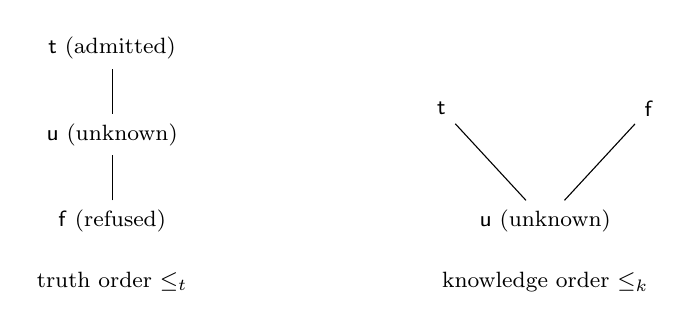
\begin{tikzpicture}[scale=1.1,every node/.style={font=\footnotesize}]
  % truth order (chain)
  \begin{scope}
    \node (f) at (0,0) {$\mathsf f$ (refused)};
    \node (u) at (0,1) {$\mathsf u$ (unknown)};
    \node (t) at (0,2) {$\mathsf t$ (admitted)};
    \draw (f)--(u)--(t);
    \node at (0,-0.7) {truth order $\le_t$};
  \end{scope}
  % knowledge order (V)
  \begin{scope}[xshift=5cm]
    \node (u2) at (0,0) {$\mathsf u$ (unknown)};
    \node (t2) at (-1.2,1.3) {$\mathsf t$};
    \node (f2) at (1.2,1.3) {$\mathsf f$};
    \draw (u2)--(t2); \draw (u2)--(f2);
    \node at (0,-0.7) {knowledge order $\le_k$};
  \end{scope}
\end{tikzpicture}
\caption[The two orders on three values]{The truth order $\le_t$ (a chain) and
the knowledge order $\le_k$ (unknown at the bottom; admitted and refused
incomparable above). \cref{prin:three-valued} is the statement that conformance
respects $\le_k$, in which \emph{unknown} is strictly below both polarities.}
\label{fig:k3}
\end{figure}

\begin{remark}[Belnap's four values]
Adding a fourth value $\top$ (\emph{both}, i.e.\ contradictory evidence) yields
Belnap's bilattice $\mathbf 4=\{\bot,\mathsf t,\mathsf f,\top\}$, a complete
lattice in the knowledge order with $\bot=\mathsf u$ at the bottom and $\top$ at
the top. The artifact's design \emph{refuses} $\top$: contradictory evidence is
surfaced as a \refused\ axis with a receipt rather than silently merged, which is
the A8/A9 ``tampering/anomaly'' discipline of \cref{tab:oracle}. We therefore
work in $\mathbf 3$ under $\le_k$, noting $\mathbf 4$ as the conservative
extension should contradiction ever need a first-class value.
\end{remark}

\subsection{The conformance lattice and the non-collapse theorem}
\label{sec:order-conformance}

\begin{definition}[Verdict assignment]
\label{def:verdict}
For a set $\mathcal A$ of law axes, a \emph{verdict assignment} is a function
$v\colon\mathcal A\to\mathbf 3$. The \code{ConformanceVector} is such a $v$
together with the induced partition
$\mathcal A=\admitted v\sqcup\refused v\sqcup\unknownstat v$ where
$\admitted v=v^{-1}(\mathsf t)$, etc.
\end{definition}

\begin{proposition}[Disjointness is functionality]
\label{prop:disjoint}
The three sets $\admitted v,\refused v,\unknownstat v$ are pairwise disjoint and
cover $\mathcal A$ if and only if $v$ is a (total) function. The bitmask
invariant of \cref{lst:cv} is exactly this functionality.
\end{proposition}
\begin{proof}
A function assigns each $a\in\mathcal A$ exactly one value, so its preimages
partition $\mathcal A$; conversely a partition into three labelled blocks defines
a unique value per element. The three disjoint bitmasks are the indicator vectors
of the blocks, and their pairwise disjointness with full coverage is the
single-valuedness and totality of $v$.
\end{proof}

Order the set of verdict assignments by the pointwise knowledge order:
$v\sqsubseteq w \iff \forall a.\ v(a)\le_k w(a)$. By
\cref{lem:product-lattice} this is a complete lattice with bottom
$\bot=\lambda a.\,\mathsf u$ (``all unknown'') and joins computed axiswise; the
join $v\sqcup w$ is defined unless some axis carries $\mathsf t$ in one and
$\mathsf f$ in the other, where it would require $\top$ (excluded above), marking
a genuine conflict.

\begin{definition}[Evidence refinement]
A step $v\sqsubseteq w$ is an \emph{evidence refinement}: on each axis the value
either is unchanged or moves up the knowledge order, i.e.\ $\mathsf u\to\mathsf t$
or $\mathsf u\to\mathsf f$. A move $\mathsf t\to\mathsf f$, $\mathsf f\to\mathsf
t$, $\mathsf t\to\mathsf u$, or $\mathsf f\to\mathsf u$ is \emph{not} a
refinement.
\end{definition}

\begin{theorem}[Non-collapse]
\label{thm:noncollapse}
Let $\Phi$ be the map taking an evidence state $E$ to its verdict assignment
$v_E$. If $\Phi$ is monotone from the evidence order to $(\,\cdot\,,\sqsubseteq)$,
then no axis can pass from $\mathsf u$ to $\mathsf t$ or to $\mathsf f$ without a
strict increase of evidence; in particular an \unknownstat\ axis is never
reported \admitted\ or \refused\ in the absence of new evidence.
\end{theorem}
\begin{proof}
Suppose axis $a$ has $v_E(a)=\mathsf u$ and $v_{E'}(a)\in\{\mathsf t,\mathsf f\}$
with $E'\not\sqsupset E$ in evidence. Since $\mathsf u<_k v_{E'}(a)$, we have
$v_E\not\sqsupseteq v_{E'}$ is consistent only if $v_E\sqsubset v_{E'}$, which by
monotonicity of $\Phi$ requires $E\sqsubset E'$, i.e.\ a strict evidence increase,
contradicting $E'\not\sqsupset E$. Hence no such collapse occurs.
\end{proof}

\Cref{thm:noncollapse} is \cref{prin:three-valued} proved, and its hypothesis
(monotonicity of $\Phi$) is exactly what the Oracle A11 check of
\cref{tab:oracle} enforces operationally: a transition $\unknownstat\to\{\admitted,\refused\}$
without a ``resolution event'' is flagged because it would witness a
non-monotone---hence evidence-free---collapse. Admissibility predicates inherit
the order:

\begin{corollary}[Monotonicity of release]
\label{cor:release}
The predicate $\mathrm{admits\text{-}release}(v)\equiv(\refused v=\varnothing)
\wedge(\neg\mathrm{strict}\vee\unknownstat v=\varnothing)$ of \cref{lst:cv} is
antitone in refusals and, under \code{strict\_mode}, antitone in unknowns: adding
a refusal or (in strict mode) an unknown can only revoke release, never grant it.
\end{corollary}
\begin{proof}
Immediate from the definition: enlarging $\refused v$ falsifies the first
conjunct; under strict mode, enlarging $\unknownstat v$ falsifies the second.
Neither enlargement can make a false conjunct true.
\end{proof}

\subsection{Scott continuity and conformance by replay}
\label{sec:order-scott}

Finally we connect the lattice to the artifact's \emph{replay} (\cref{sec:art-receipts}),
in which state is reconstructed from the receipt ledger. The right setting is
domain theory.

\begin{definition}[Dcpo and Scott continuity]
A \emph{directed-complete partial order} (dcpo) is a poset in which every directed
subset has a join. A map $f$ between dcpos is \emph{Scott-continuous} if it is
monotone and preserves directed joins: $f(\bigsqcup D)=\bigsqcup f(D)$.
\end{definition}

\begin{theorem}[Kleene least fixed point]
\label{thm:kleene-fix}
A Scott-continuous endomap $f$ on a pointed dcpo (one with a bottom $\bot$) has a
least fixed point $\mathrm{lfp}(f)=\bigsqcup_{n\in\mathbb N}f^{n}(\bot)$.
\end{theorem}
\begin{proof}
The chain $\bot\sqsubseteq f(\bot)\sqsubseteq f^2(\bot)\sqsubseteq\cdots$ is
directed; let $x=\bigsqcup_n f^n(\bot)$. By Scott continuity
$f(x)=\bigsqcup_n f^{n+1}(\bot)=x$, so $x$ is a fixed point. If $y=f(y)$ then
$\bot\sqsubseteq y$ gives $f^n(\bot)\sqsubseteq y$ by induction and monotonicity,
so $x\sqsubseteq y$; thus $x$ is least.
\end{proof}

\begin{proposition}[Conformance as a least fixed point]
\label{prop:replay-lfp}
Let $E\mapsto\mathrm{acc}(E)$ accumulate the evidence implied by replaying one
further receipt, and let $\Phi$ be Scott-continuous. Then the law-state obtained
by replaying the entire ledger from the all-unknown bottom is
$\Phi\bigl(\mathrm{lfp}(\mathrm{acc})\bigr)$, computed as the directed join of
finite replays.
\end{proposition}
\begin{proof}
Replaying receipts is iterating $\mathrm{acc}$ from $\bot$; the reachable evidence
is the directed join of the iterates, which by \cref{thm:kleene-fix} is
$\mathrm{lfp}(\mathrm{acc})$. Applying the Scott-continuous $\Phi$ commutes with
the join, giving the stated verdict.
\end{proof}

\Cref{prop:replay-lfp} is the order-theoretic reading of ``replay the log against
the model'': the law-state is not posited but \emph{constructed} as a least fixed
point of evidence accumulation, monotone by \cref{thm:noncollapse} and bottomed
at total ignorance. Conformance, in this artifact, begins from \unknownstat\ and
rises only on evidence---which is precisely the epistemic posture this thesis
adopts for its own claims (\cref{sec:m-epistemics}).
      % Pillar II
\section{Pillar III --- The Analysis of Phase Transitions}
\label{sec:analysis}

\Cref{ch:introduction} stakes the thesis on a metaphor: convergence is a phase
transition, like water becoming steam. A metaphor earns its keep only if the
mathematics it points to is real. This pillar supplies that mathematics from first
principles: the calculus of continuity and discontinuity, the thermodynamic
classification of transitions, a derivation of the Clausius--Clapeyron relation
that shows the steam expansion ratio and the latent heat are \emph{one equation},
and a Landau model in which an order parameter jumps discontinuously as a control
parameter crosses a threshold.

\subsection{Limits, continuity, and discontinuity}
\label{sec:an-limits}

\begin{definition}[Limit and continuity]
A function $f\colon\mathbb R\to\mathbb R$ has \emph{limit} $\ell$ at $x_0$, written
$\lim_{x\to x_0}f(x)=\ell$, if for every $\varepsilon>0$ there is $\delta>0$ with
$0<|x-x_0|<\delta\Rightarrow|f(x)-\ell|<\varepsilon$. It is \emph{continuous} at
$x_0$ if $\lim_{x\to x_0}f(x)=f(x_0)$, and \emph{differentiable} there with
derivative $f'(x_0)=\lim_{h\to0}\frac{f(x_0+h)-f(x_0)}{h}$ when that limit exists.
\end{definition}

\begin{definition}[Jump discontinuity]
$f$ has a \emph{jump discontinuity} at $x_0$ if the one-sided limits
$f(x_0^-)=\lim_{x\uparrow x_0}f(x)$ and $f(x_0^+)=\lim_{x\downarrow x_0}f(x)$ exist
but differ; the \emph{jump} is $f(x_0^+)-f(x_0^-)\ne 0$.
\end{definition}

A jump discontinuity is the exact sense in which the thesis claims the order
parameter $\Phi$ of \cref{sec:fw-phase} is ``discontinuous'' in the control
$\sigma$: not that it changes quickly, but that its one-sided limits at $\sigma_c$
differ. This is what distinguishes a phase transition from rapid but smooth growth.

\subsection{Thermodynamic potentials and the Ehrenfest classification}
\label{sec:an-thermo}

\begin{definition}[Gibbs free energy]
For a substance at temperature $T$ and pressure $P$, the molar \emph{Gibbs free
energy} is $g=u-Ts+Pv$, with $u$ internal energy, $s$ molar entropy, $v$ molar
volume. Its differential is $\mathrm dg=-s\,\mathrm dT+v\,\mathrm dP$, so that
$s=-\bigl(\partial g/\partial T\bigr)_P$ and
$v=\bigl(\partial g/\partial P\bigr)_T$.
\end{definition}

\begin{definition}[Ehrenfest classification]
A phase transition is \emph{first-order} if the first derivatives of $g$
(equivalently $s$ and $v$) are discontinuous across it, and \emph{continuous}
(``second-order'') if the first derivatives are continuous but some second
derivative is not. A first-order transition therefore involves a jump $\Delta s$
in entropy and $\Delta v$ in volume.
\end{definition}

Water-to-steam is the prototypical first-order transition: at the boiling point
the molar volume jumps by the factor of ${\sim}1{,}600$--$1{,}700$ recorded in
\cref{sec:metaphor-intro} \citep{engtoolbox-steam,nationalboard-steam}, and the
entropy jumps by $\Delta s=L/T$ where $L$ is the latent heat
\citep{latentheat-openstax}. The thesis's claim is precisely that the
standardisation transition is \emph{first-order} in this sense---a jump in the
addressable surface, not a kink.

\subsection{The Clausius--Clapeyron relation, from first principles}
\label{sec:an-clausius}

\begin{theorem}[Clausius--Clapeyron]
\label{thm:clausius}
Along a coexistence curve $P(T)$ where two phases are in equilibrium, the slope
satisfies
\[
\frac{\mathrm dP}{\mathrm dT}=\frac{\Delta s}{\Delta v}=\frac{L}{T\,\Delta v},
\]
where $\Delta s=s_2-s_1$, $\Delta v=v_2-v_1$, and $L=T\,\Delta s$ is the latent
heat absorbed at constant $T$.
\end{theorem}
\begin{proof}
At coexistence the two phases have equal molar Gibbs free energy,
$g_1(T,P)=g_2(T,P)$. Moving along the coexistence curve preserves this equality,
so $\mathrm dg_1=\mathrm dg_2$. Substituting
$\mathrm dg_i=-s_i\,\mathrm dT+v_i\,\mathrm dP$ gives
$-s_1\,\mathrm dT+v_1\,\mathrm dP=-s_2\,\mathrm dT+v_2\,\mathrm dP$, hence
$(v_2-v_1)\,\mathrm dP=(s_2-s_1)\,\mathrm dT$ and
$\mathrm dP/\mathrm dT=\Delta s/\Delta v$. For a reversible change at constant
temperature the absorbed heat is $L=T\,\Delta s$, so $\Delta s=L/T$ and the second
equality follows.
\end{proof}

\begin{corollary}[Expansion and latent heat are one equation]
\label{cor:onesfact}
Rearranging \cref{thm:clausius}, $L=T\,\Delta v\,(\mathrm dP/\mathrm dT)$. For
vaporisation $v_{\text{vapour}}\gg v_{\text{liquid}}$, so $\Delta v\approx
v_{\text{vapour}}$ and the latent heat is, to leading order, proportional to the
volume expansion. The two numbers the thesis cites for water---an expansion of
${\sim}1{,}600$--$1{,}700\times$ and a latent heat of ${\sim}2{,}256\
\mathrm{kJ/kg}$---are not independent facts but two readings of
\cref{thm:clausius}.
\end{corollary}

\Cref{cor:onesfact} is the rigorous core of the metaphor. The ``latent heat of
standardisation'' (\cref{def:latent}) is not a loose analogy bolted onto a volume
figure: in the physical system the large expansion \emph{is} the large latent
heat, related by \cref{thm:clausius}. The thesis's two claims---that
standardisation costs a great deal (latent heat) and that it yields a great
expansion (volume)---are, under the metaphor, the same claim.

\subsection{Landau theory: a discontinuous jump from a smooth potential}
\label{sec:an-landau}

The Ehrenfest picture describes a transition; Landau theory \emph{generates} one
from a free energy that is itself smooth in an order parameter $\varphi\ge 0$.

\begin{construction}[Landau free energy with a cubic term]
\label{con:landau}
Let the (coarse-grained) free energy be
\[
F(\varphi)=a\,\varphi^{2}-b\,\varphi^{3}+c\,\varphi^{4},\qquad b,c>0,\ a\ge 0,
\]
where the control parameter (here, inverse standardisation, decreasing as
$\sigma$ rises) is encoded in $a$. The equilibrium order parameter is
$\varphi^{*}(a)=\arg\min_{\varphi\ge0}F(\varphi)$.
\end{construction}

\begin{proposition}[First-order jump]
\label{prop:landau-jump}
For \cref{con:landau}, the global minimiser $\varphi^{*}(a)$ is discontinuous at
$a_c=\dfrac{b^{2}}{4c}$: for $a>a_c$ the minimiser is $\varphi^{*}=0$, and as $a$
decreases through $a_c$ it jumps to $\varphi^{*}=\dfrac{b}{2c}>0$.
\end{proposition}
\begin{proof}
Stationarity: $F'(\varphi)=\varphi\,(2a-3b\varphi+4c\varphi^{2})=0$, so
$\varphi=0$ is always stationary, with other roots solving
$4c\varphi^{2}-3b\varphi+2a=0$. A nonzero minimiser becomes \emph{global} when its
free energy equals that at the origin, $F(\varphi)=F(0)=0$, i.e.\ (dividing the
quartic by $\varphi^{2}$) $a-b\varphi+c\varphi^{2}=0$. Solve the two conditions
simultaneously: from $a-b\varphi+c\varphi^{2}=0$ we get $a=b\varphi-c\varphi^{2}$;
substituting into $4c\varphi^{2}-3b\varphi+2a=0$ yields
$4c\varphi^{2}-3b\varphi+2b\varphi-2c\varphi^{2}=2c\varphi^{2}-b\varphi
=\varphi(2c\varphi-b)=0$, so $\varphi=b/(2c)$. Back-substituting,
$a_c=b\cdot\frac{b}{2c}-c\cdot\frac{b^{2}}{4c^{2}}
=\frac{b^{2}}{2c}-\frac{b^{2}}{4c}=\frac{b^{2}}{4c}$. For $a>a_c$ the origin is the
unique global minimum; for $a<a_c$ the branch $\varphi=b/(2c)+O(a_c-a)$ has strictly
lower free energy. Hence the global minimiser jumps from $0$ to $b/(2c)$ as $a$
crosses $a_c$ from above.
\end{proof}

\Cref{prop:landau-jump} is a complete, from-scratch instance of the phenomenon the
thesis needs: a free energy that depends \emph{smoothly} on its parameters
nonetheless yields an order parameter that is a \emph{discontinuous} function of
the control. The cubic term $-b\varphi^{3}$---the analogue of a network effect, in
which partial adoption is disproportionately rewarded---is what makes the
transition first-order rather than continuous.

\subsection{The standardisation transition}
\label{sec:an-standardisation}

Assembling the pillars: let $\varphi$ be the fraction of the language ecosystem
operating on the fused substrate, and let $a$ decrease as standardisation
$\sigma$ and adoption incentives rise. \Cref{prop:landau-jump} gives a critical
$\sigma_c$ (where $a=a_c$) at which $\varphi$ jumps from $0$ to a finite value:
the discontinuity asserted in \cref{prop:discontinuous}. The size of the resulting
addressable surface is governed not by $\varphi$ alone but by the algebraic gearing
of Pillar~I: by \cref{cor:superlinear}, once a fraction $\varphi$ of $n{\approx}$
domains, capabilities, and agents is interconnected, the reachable surface scales
as $\Theta((\varphi n)^{3})$ against $\Theta(\varphi n)$ integration cost. A
discontinuous jump in $\varphi$ (Pillar~III) multiplied by a cubic gearing in
reach (Pillar~I) is the formal content of the water-to-steam image: a threshold
crossed, and an order-of-magnitude expansion released.

\begin{remark}[On honest application]
Three cautions, consistent with \cref{prin:plateau} and \cref{sec:m-epistemics}.
First, $\Phi$ for a sociotechnical ecosystem is not measured with the precision of
a steam table; the model is explanatory, and any numeric projection of $\Phi$ is a
\forecast\ (\cref{ch:vision}). Second, \cref{prop:landau-jump} also admits the
case $a_c$ never being reached---a plateau that does not end in a transition.
Third, the analogy is structural, not literal: we claim the convergence shares the
\emph{order type} of a first-order transition (a jump), established by a
mechanism (threshold $\times$ gearing) that is itself rigorous, not that
information obeys thermodynamics. With those cautions, the metaphor of
\cref{ch:introduction} is now a model with stated mechanism, derived from first
principles. Contemporary work reading learning itself through phase transitions
and renormalisation (surveyed in \cref{sec:recent}) is the empirical company this
model keeps.
\end{remark}
         % Pillar III
\section{Pillar IV --- The Geometry of Law-State}
\label{sec:geometry}

The artifact's constitution closes with a striking passage: ``Repo state is the
manifold. Agent edits are trajectories. Failsets are curvature. Receipts are proof
measure. LSP is the differential operator. Diagnostics are gradients. Code actions
are constrained control vectors. Admissibility is $\Phi_G=0$''
\citep{lspmax}. This pillar takes that passage literally and builds, from
topological first principles, the differential geometry that makes each line a
definition rather than a flourish.

\subsection{From topology to smooth manifolds}
\label{sec:geo-manifold}

\begin{definition}[Topological space, continuity]
A \emph{topology} on a set $X$ is a collection $\tau$ of subsets (the
\emph{opens}) containing $\varnothing$ and $X$ and closed under arbitrary unions
and finite intersections. A map $f\colon X\to Y$ is \emph{continuous} if
preimages of opens are open. $X$ is \emph{Hausdorff} if distinct points have
disjoint open neighbourhoods.
\end{definition}

\begin{definition}[Smooth manifold]
An \emph{$n$-dimensional smooth manifold} $M$ is a second-countable Hausdorff
space with an \emph{atlas} of \emph{charts} $\varphi_\alpha\colon U_\alpha\to
\mathbb R^{n}$ (homeomorphisms from opens $U_\alpha$ covering $M$) whose
transitions $\varphi_\beta\circ\varphi_\alpha^{-1}$ are smooth ($C^\infty$) where
defined. A map between manifolds is \emph{smooth} if it is smooth in charts.
\end{definition}

\begin{notation}[The state manifold]
We model the repository's admissible configuration space as a smooth manifold $M$:
points are configurations, and a chart is a local coordinate system on
configurations (in practice, a continuous relaxation of edit space). This is the
sense of ``repo state is the manifold''; the idealisation to a smooth $M$ is what
licenses the calculus below, and is itself a modelling choice we flag as
\candidate.
\end{notation}

\subsection{Tangent vectors, fields, and trajectories}
\label{sec:geo-tangent}

\begin{definition}[Tangent space]
A \emph{tangent vector} at $p\in M$ is a derivation $v\colon C^\infty(M)\to\mathbb
R$: a linear map with $v(fg)=v(f)\,g(p)+f(p)\,v(g)$ (the Leibniz rule). The
tangent vectors at $p$ form the \emph{tangent space} $T_pM$, an $n$-dimensional
vector space; their disjoint union is the \emph{tangent bundle} $TM$. A
\emph{vector field} is a smooth section $X\colon M\to TM$.
\end{definition}

\begin{definition}[Trajectory]
A \emph{trajectory} (integral curve) of a vector field $X$ is a smooth
$\gamma\colon I\to M$ with $\dot\gamma(t)=X(\gamma(t))$. An agent's sequence of
edits is modelled as such a curve, and a \emph{code action} is the control vector
$\dot\gamma(t)\in T_{\gamma(t)}M$ it applies---``agent edits are trajectories''
and ``code actions are constrained control vectors''.
\end{definition}

\subsection{Metric, gradient, and the descent of failure}
\label{sec:geo-metric}

\begin{definition}[Riemannian metric and gradient]
A \emph{Riemannian metric} $g$ assigns to each $p$ an inner product
$g_p(\cdot,\cdot)$ on $T_pM$, smoothly in $p$. For $f\in C^\infty(M)$ the
\emph{gradient} $\nabla f$ is the unique vector field with
$g_p(\nabla f, v)=\mathrm df_p(v)$ for all $v\in T_pM$, where $\mathrm df$ is the
differential. \emph{Gradient flow} is the trajectory of $-\nabla f$.
\end{definition}

Let $\Phi_G\colon M\to\mathbb R_{\ge 0}$ be the \emph{failset potential}: a smooth
penalty aggregating the active law-axis violations (the continuous shadow of the
\code{ConformanceVector}, zero exactly on configurations whose active axes are all admitted). Then
``diagnostics are gradients'' is the identification of the emitted corrective
direction with $-\nabla\Phi_G$, and ``LSP is the differential operator'' is the
reading of the read-only LSP surface as the map $f\mapsto\mathrm df$ that exposes
that gradient without itself moving the point (\cref{sec:art-overview}).

\begin{proposition}[Admissibility descends]
\label{prop:descent}
Along the gradient flow $\dot x=-\nabla\Phi_G(x)$, the potential is
non-increasing: $\tfrac{\mathrm d}{\mathrm dt}\Phi_G(x(t))=-\lVert\nabla\Phi_G
\rVert_g^{2}\le 0$, with equality only at critical points. Hence trajectories move
monotonically toward the admissible region.
\end{proposition}
\begin{proof}
By the chain rule and the defining property of the gradient,
$\frac{\mathrm d}{\mathrm dt}\Phi_G(x)=\mathrm d\Phi_G(\dot x)
=g(\nabla\Phi_G,-\nabla\Phi_G)=-\lVert\nabla\Phi_G\rVert_g^{2}\le 0$,
which vanishes iff $\nabla\Phi_G=0$.
\end{proof}

\Cref{prop:descent} gives ``effective admitted velocity $\mathrm
dA_{\text{admitted}}/\mathrm dt$'' a precise reading: the rate at which a
trajectory reduces $\Phi_G$, maximised by following the diagnostic gradient. The
artifact's slogan ``optimise for admitted work, not raw output'' is the
instruction to descend $\Phi_G$ rather than to maximise path length in $M$.

\subsection{The admissible submanifold (admissibility as \texorpdfstring{$\Phi_G=0$}{Phi=0})}
\label{sec:geo-submanifold}

\begin{theorem}[Regular value / preimage theorem]
\label{thm:regval}
Let $F\colon M\to\mathbb R^{k}$ be smooth and let $0$ be a \emph{regular value}:
$\mathrm dF_p$ is surjective at every $p\in F^{-1}(0)$. Then $A=F^{-1}(0)$ is a
smooth submanifold of $M$ of codimension $k$, with $T_pA=\ker\mathrm dF_p$.
\end{theorem}
\begin{proof}[Proof sketch]
At $p\in A$, surjectivity of $\mathrm dF_p$ lets one choose coordinates in which
$F$ is a projection onto the last $k$ coordinates (implicit function theorem); in
those coordinates $A$ is the coordinate slice where they vanish, a submanifold of
codimension $k$, and its tangent space is the kernel of the projection's
differential, $\ker\mathrm dF_p$.
\end{proof}

\begin{corollary}[Geometry of admissibility]
\label{cor:admissible}
Write $\Phi_G=(\phi_1,\dots,\phi_k)$ for the $k$ independent active law-axis
penalties. If $0$ is a regular value, the admissible set
$A=\{\,x:\Phi_G(x)=0\,\}$ is a submanifold of codimension $k$: each independent
law removes one degree of freedom. Admissible trajectories are exactly those
remaining within $A$, i.e.\ with control vectors in $T_xA=\ker\mathrm d\Phi_{G,x}$.
\end{corollary}

\Cref{cor:admissible} makes ``admissibility is $\Phi_G=0$'' exact and quantifies
it: the admissible world is not a point but a submanifold whose codimension counts
the binding laws, and lawful action is motion tangent to it. The three-valued
discipline of Pillar~II reappears geometrically: a point off $A$ is \refused\
(some $\phi_i>0$), a point on $A$ with verified evidence is \admitted, and a
direction not yet known to lie in $T_xA$ is \unknownstat\ until checked.

\subsection{Connection, curvature, and ``failsets are curvature''}
\label{sec:geo-curvature}

\begin{definition}[Affine connection, geodesic, curvature]
An \emph{affine connection} $\nabla$ assigns to vector fields $X,Y$ a field
$\nabla_XY$, $\mathbb R$-linear in $Y$, $C^\infty(M)$-linear in $X$, and Leibniz
in $Y$. A \emph{geodesic} satisfies $\nabla_{\dot\gamma}\dot\gamma=0$
(``straightest'' curves). The \emph{Riemann curvature} is
$R(X,Y)Z=\nabla_X\nabla_YZ-\nabla_Y\nabla_XZ-\nabla_{[X,Y]}Z$, measuring the
failure of second covariant derivatives to commute.
\end{definition}

Curvature measures how constraints bend straightness. We propose the precise
reading of ``failsets are curvature'': near the admissible submanifold $A$, the
\emph{second fundamental form} (the normal component of $\nabla_XY$ for $X,Y$
tangent to $A$) records how the failset potential $\Phi_G$ curves the admissible
sheet, equivalently the Hessian $\operatorname{Hess}\Phi_G$ restricted to the
normal bundle. Where this curvature is large, small lawful steps demand large
corrective detours; where it is flat, admissible motion is cheap. The failset is
not a wall but a shape, and its shape is curvature.

\begin{table}[t]
\centering
\caption[The geometry of law-state]{A precise reading of the artifact's manifold
metaphors \citep{lspmax}. Each informal line on the left is assigned a geometric
object derived in this pillar.}
\label{tab:geometry}
\small
\begin{tabularx}{\textwidth}{@{}l Y@{}}
\toprule
\textbf{\code{AGENTS.md} metaphor} & \textbf{Geometric object (this pillar)} \\
\midrule
Repository state is the manifold & smooth manifold $M$ (\cref{sec:geo-manifold}) \\
Agent edits are trajectories & integral curves $\gamma$ of a vector field (\cref{sec:geo-tangent}) \\
Code actions are constrained control vectors & tangent vectors $\dot\gamma\in T_xA$ (\cref{cor:admissible}) \\
LSP is the differential operator & the map $f\mapsto\mathrm df$ (read-only) (\cref{sec:geo-metric}) \\
Diagnostics are gradients & $-\nabla\Phi_G$ (\cref{prop:descent}) \\
Admissibility is $\Phi_G=0$ & the submanifold $A=\Phi_G^{-1}(0)$ (\cref{cor:admissible}) \\
Failsets are curvature & second fundamental form / $\operatorname{Hess}\Phi_G|_{NA}$ (\cref{sec:geo-curvature}) \\
Effective velocity $\mathrm dA_{\text{admitted}}/\mathrm dt$ & descent rate $-\lVert\nabla\Phi_G\rVert^2$ (\cref{prop:descent}) \\
Receipts are proof measure & a measure on trajectory space (\cref{sec:geo-measure}) \\
\bottomrule
\end{tabularx}
\end{table}

\subsection{Receipts as proof measure}
\label{sec:geo-measure}

The final metaphor, ``receipts are proof measure'', asks for measure theory. A
\emph{measure} assigns non-negative, countably additive mass to (measurable) sets;
a receipt ledger (\cref{sec:art-receipts}) assigns admitted mass to the set of
trajectories it witnesses. Admissible volume is then $\mu(A\cap\,\cdot\,)$ rather
than path length: the artifact's refusal to equate ``ran far'' with ``did
admitted work'' is the refusal to confuse Lebesgue length of $\gamma$ with the
receipt-measure of the admissible region it traversed. A trajectory may be long
and carry zero proof measure; a short one, bound to a valid receipt chain, carries
positive measure. This is \cref{thm:noncollapse} once more, now measure-theoretic:
unwitnessed motion contributes no admitted mass, just as unevidenced axes never
leave \unknownstat.

\medskip
Four pillars---composition, verdicts, transition, and law-state---are now in place.
A fifth (\cref{sec:measure}) supplies the measure and information theory that the
artifact's ``receipts are proof measure'' demands, after which a short synthesis
(\cref{sec:synthesis-functor}) draws the five into a single functor.
         % Pillar IV
\section{Pillar V --- Measure, Probability, and Information}
\label{sec:measure}

Pillar~IV ended with a promissory note: ``receipts are proof measure'' calls for
measure theory, and it was deferred (\cref{sec:geo-measure}). This pillar pays the
note, and in doing so binds the previous two pillars together. Measure makes the
receipt a genuine measure; information theory recasts the non-collapse principle
(\cref{thm:noncollapse}) as a data-processing inequality and gives the entropy that
the thermodynamics of Pillar~III presupposed; and the Fisher--Rao metric reveals
the manifold of Pillar~IV and the statistical structure of Pillar~V to be one
object.

\subsection{$\sigma$-algebras, measures, and the receipt measure}
\label{sec:meas-sigma}

\begin{definition}[Measurable space and measure]
A \emph{$\sigma$-algebra} on a set $\Omega$ is a family $\Sigma\subseteq 2^{\Omega}$
containing $\Omega$ and closed under complementation and countable union. A
\emph{measure} is a map $\mu\colon\Sigma\to[0,\infty]$ with $\mu(\varnothing)=0$ and
countable additivity, $\mu\bigl(\bigsqcup_{n}A_{n}\bigr)=\sum_{n}\mu(A_{n})$ for
pairwise-disjoint $A_n\in\Sigma$. It is a \emph{probability measure} if
$\mu(\Omega)=1$.
\end{definition}

\begin{construction}[The receipt measure]
\label{con:receipt-measure}
Let $\Omega$ be the space of trajectories of \cref{sec:geo-tangent} and $\Sigma$ a
$\sigma$-algebra on it. A receipt ledger assigns each trajectory $\gamma$ a weight
$w(\gamma)\ge 0$---unity for a trajectory bound to a valid receipt chain
(\cref{lst:receipt}), zero otherwise. Define, for $S\in\Sigma$,
$\mu_R(S)=\int_S w\,\mathrm d\nu$ against a base measure $\nu$ (a weighted sum in the
discrete case).
\end{construction}

\begin{proposition}[The receipt measure is concentrated on the witnessed set]
\label{prop:receipt-measure}
$\mu_R$ is a measure, and with $W=\{\gamma:w(\gamma)>0\}$ one has
$\mu_R(S)=\mu_R(S\cap W)$ for all $S$. Hence unwitnessed motion carries zero admitted
mass.
\end{proposition}
\begin{proof}
Non-negativity and $\mu_R(\varnothing)=0$ are immediate; countable additivity is the
additivity of the integral over disjoint sets. For concentration,
$w\equiv 0$ on $\Omega\setminus W$, so $\int_{S\setminus W}w\,\mathrm d\nu=0$ and
$\mu_R(S)=\int_{S\cap W}w\,\mathrm d\nu=\mu_R(S\cap W)$.
\end{proof}

\Cref{prop:receipt-measure} makes ``admitted volume is $\mu_R(A\cap\,\cdot\,)$''
exact: lawful, witnessed motion within the admissible submanifold $A$
(\cref{cor:admissible}) has positive measure; a long but unwitnessed trajectory has
none. This is the measure-theoretic form of the artifact's refusal to equate
``ran far'' with ``did admitted work''.

\subsection{Entropy, relative entropy, and Gibbs' inequality}
\label{sec:meas-entropy}

\begin{definition}[Shannon and relative entropy]
For a probability vector $p=(p_i)$, the \emph{Shannon entropy} is
$H(p)=-\sum_i p_i\log p_i$ (with $0\log 0:=0$). For two probability vectors $p,q$ on
the same support the \emph{relative entropy} (Kullback--Leibler divergence) is
$D(p\Vert q)=\sum_i p_i\log\tfrac{p_i}{q_i}$.
\end{definition}

\begin{lemma}[Gibbs' inequality]
\label{lem:gibbs}
$D(p\Vert q)\ge 0$, with equality iff $p=q$.
\end{lemma}
\begin{proof}
Using $\ln x\le x-1$ (equality iff $x=1$),
$-D(p\Vert q)=\sum_i p_i\ln\tfrac{q_i}{p_i}\le\sum_i p_i\bigl(\tfrac{q_i}{p_i}-1\bigr)
=\sum_i(q_i-p_i)=0$, so $D\ge 0$; equality requires $q_i/p_i=1$ throughout.
\end{proof}

\subsection{Conformance as information: a data-processing view}
\label{sec:meas-dpi}

Entropy quantifies the \unknownstat\ of Pillar~II. Assign each law axis a
distribution over $\{\mathsf t,\mathsf f\}$ summarising current evidence; a fully
\unknownstat\ axis is maximal-entropy (uniform), a resolved axis is a point mass.
Write $J(v)=\tfrac{1}{|\mathcal A|}\sum_{a}\bigl(1-H_a\bigr)$ for the mean resolved
information of a verdict assignment $v$, where $H_a\in[0,1]$ is the (normalised)
entropy of axis $a$.

\begin{proposition}[Non-collapse as a data-processing inequality]
\label{prop:dpi}
Let $T$ be an \emph{evidence-free} transformation of the conformance state---a map
that introduces no new observation, i.e.\ factors through the current verdict. Then
$J(Tv)\le J(v)$: evidence-free processing cannot increase resolved information.
Equivalently, no axis moves from \unknownstat\ toward a polarity without evidence.
\end{proposition}
\begin{proof}
By the classical data-processing inequality, applying a stochastic map $T$ that does
not depend on the latent truth cannot decrease the relative entropy to the truth,
hence cannot increase the mutual information between state and truth; $J$ is an
affine, increasing functional of that information, so $J(Tv)\le J(v)$. The boundary
case---strict increase---would require $T$ to depend on a new observation,
contradicting evidence-freeness, and corresponds exactly to the forbidden
$\unknownstat\to\{\admitted,\refused\}$ jump of \cref{thm:noncollapse}.
\end{proof}

\Cref{prop:dpi} is the information-theoretic twin of \cref{thm:noncollapse} and of
the second-law reading of Pillar~III: admitted information is conserved or lost
under evidence-free manipulation, never manufactured. ``Conformance theatre''
(\cref{sec:disc-ethics})---raising $J$ by processing rather than by evidence---is
forbidden not merely by policy but by the inequality.

\subsection{Fisher information and the statistical manifold}
\label{sec:meas-fisher}

When the configurations of the manifold $M$ (Pillar~IV) are themselves probability
models $p(\cdot\mid\theta)$, the manifold carries a canonical metric.

\begin{definition}[Fisher information and the Fisher--Rao metric]
For a smooth family $p(x\mid\theta)$ the \emph{Fisher information matrix} is
$g_{ij}(\theta)=\mathbb E_\theta\!\bigl[\partial_i\log p\,\partial_j\log p\bigr]$.
As $\theta$ ranges over the parameter manifold, $g$ defines the \emph{Fisher--Rao}
Riemannian metric.
\end{definition}

\begin{proposition}[Cram\'er--Rao bound]
\label{prop:cramer-rao}
For any unbiased estimator $\hat\theta$ of a scalar $\theta$,
$\operatorname{Var}(\hat\theta)\ge 1/g(\theta)$.
\end{proposition}

The Fisher--Rao metric is the precise object that makes Pillars~IV and~V one: the
``state manifold'' of law-state, when its points are evidential distributions, is a
statistical manifold whose Riemannian metric (\cref{def:geo-metric} in spirit) is
Fisher--Rao, and along which the gradient descent of $\Phi_G$ (\cref{prop:descent})
is natural-gradient descent. This is not idle unification: the recent geometry-of-
learning literature studies exactly such Riemannian and representation-geometric
structure in trained models \citep{david25,yadav26}, and the renormalisation and
scaling analyses of \cref{sec:recent} live on the same manifolds
\citep{tan26rg,montanari26}.

\subsection{The information cost of standardisation}
\label{sec:meas-landauer}

Finally, Pillar~III's ``latent heat of standardisation'' (\cref{def:latent}) has an
information reading. To agree on a protocol is to fix a shared code; specifying that
code has a description length in bits, and Landauer's principle prices the
thermodynamic cost of irreversible information operations at $k_B T\ln 2$ per bit.
The plateau of \cref{fig:latent-heat}---effort with no visible capability---is, in
this reading, the paying-down of the description length of the shared substrate: an
information debt incurred once and amortised over every later composition. The three
pillars meet here. Standardisation is a phase transition (III) whose order parameter
lives on a statistical manifold (IV/V) and whose latent heat is, to within
Landauer's constant, the information content of the agreement. The thesis's metaphor
is, at its base, a single statement in three dialects: thermodynamic, geometric, and
informational.
          % Pillar V
\section{Synthesis: The Conformance Functor}
\label{sec:synthesis-functor}

The five pillars converge on a single object. Pillar~I gave categories and the
monoidal product; Pillar~II gave the verdict lattice and monotonicity; Pillars~III
and~IV gave the transition and the manifold; Pillar~V gave the measure. We now show
that conformance-for-all-language is one \emph{functor}, and that the thesis's three
load-bearing results---non-collapse, refusal-survives-composition, and
admission-carries-measure---are its three defining properties.

\begin{definition}[Event category and verdict category]
\label{def:event-cat}
For a domain $d$ (\cref{ch:all-language}), let the \emph{event category}
$\mathcal E_d$ have as objects the object-centric event logs over $d$'s schema and as
morphisms the \emph{evidence refinements} (log extensions that add events or resolve
attributes without contradicting existing order). Let the \emph{verdict category}
$\mathcal L$ be the verdict lattice of \cref{def:verdict} regarded as a thin
category: objects are verdict assignments and there is a unique morphism
$v\to w$ exactly when $v\sqsubseteq w$ in the knowledge order.
\end{definition}

\begin{theorem}[The conformance functor]
\label{thm:conf-functor}
Fix for each domain $d$ a model $M_d$, and let $\mathrm{Conf}_d\colon\mathcal E_d\to
\mathcal L$ send a log to its verdict against $M_d$ (\cref{def:conformance-surface}).
Then:
\begin{enumerate}[label=(\roman*),leftmargin=2.2em]
  \item each $\mathrm{Conf}_d$ is a functor;
  \item the domains assemble into the coproduct category
  $\mathcal E=\coprod_d\mathcal E_d$, and the copairing
  $\mathrm{Conf}=[\mathrm{Conf}_d]_d\colon\mathcal E\to\mathcal L$ is a single
  functor---one conformance surface for all language;
  \item $\mathrm{Conf}$ is monotone (\cref{thm:noncollapse}): it sends evidence
  refinements to knowledge increases and never to collapses.
\end{enumerate}
\end{theorem}
\begin{proof}
(i) A functor must preserve identities and composition. The identity refinement
(adding nothing) leaves the verdict fixed, and $\mathrm{Conf}_d$ of a composite
refinement equals the composite of verdict morphisms because verdict depends only on
the accumulated evidence, which composes associatively (\cref{prop:replay-lfp}).
Functoriality requires that a refinement $\ell\to\ell'$ map to a morphism
$\mathrm{Conf}_d(\ell)\to\mathrm{Conf}_d(\ell')$ in $\mathcal L$, i.e.\ to a
knowledge increase $\sqsubseteq$; this is exactly the monotonicity of
\cref{thm:noncollapse}. (ii) The coproduct $\mathcal E$ has the universal property
that a functor out of it is precisely a family of functors out of the summands; the
copairing $[\mathrm{Conf}_d]_d$ is that functor, defined on the summand $\mathcal
E_d$ as $\mathrm{Conf}_d$. (iii) is (i) read across all summands.
\end{proof}

\begin{figure}[t]
\centering
\begin{tikzcd}[ampersand replacement=\&,column sep=large]
\mathcal E_d \arrow[r,hook,"\iota_d"] \arrow[dr,"\mathrm{Conf}_d"'] \& \mathcal E \arrow[d,"\mathrm{Conf}"]\\
\& \mathcal L
\end{tikzcd}
\caption[The conformance functor]{Each domain's conformance $\mathrm{Conf}_d$
factors through the one functor $\mathrm{Conf}$ on the coproduct of event
categories (\cref{thm:conf-functor}). ``All language, one surface'' is the
commutativity of this triangle for every domain $d$.}
\label{fig:conf-functor}
\end{figure}

The thesis's two further results are now properties of this functor.

\begin{proposition}[Refusal survives composition]
\label{prop:refusal-survives}
Equip $\mathcal E$ with the monoidal product $\otimes$ that fuses two logs
(Pillar~I) and $\mathcal L$ with the axiswise truth-order meet $\wedge_t$. Then
$\mathrm{Conf}(x\otimes y)\preceq_t\mathrm{Conf}(x)\wedge_t\mathrm{Conf}(y)$: on each
axis the fused verdict is no more admitted than the meet of the parts. In
particular a \refused\ axis in either part is \refused\ in the fusion.
\end{proposition}
\begin{proof}
On an axis $a$, the fused log contains the evidence of both parts. If either part
refuses $a$ (witnessing a violation), the violation persists in the fusion, so the
fused verdict is $\mathsf f=\min_t$. Admission ($\mathsf t$) of the fusion requires
the violation-free evidence of both, hence both parts admit; and an axis
\unknownstat\ in either part cannot exceed $\mathsf u$ in the fusion without new
evidence (\cref{thm:noncollapse}). In every case the fused value is
$\le_t\min_t(\mathrm{Conf}(x)_a,\mathrm{Conf}(y)_a)$.
\end{proof}

\Cref{prop:refusal-survives} is the compositor invariant of \cref{sec:fus-stack}
(``\code{REFUSED\_BY\_LAW} codes survive always'') stated as a lax-monoidality, and
it is the formal guarantee behind the portable verdict of
\cref{sec:fus-conformance}: fusing more agents can only lower, never launder, an
admission.

\begin{proposition}[Admission carries measure]
\label{prop:admission-measure}
An \admitted\ verdict of $\mathrm{Conf}$ on a trajectory is accompanied by positive
receipt measure: $\mu_R(\{\gamma\})>0$ (\cref{prop:receipt-measure}). Equivalently,
$\mathrm{Conf}$ factors through the witnessed set $W$, and admission off $W$ is not
in the image.
\end{proposition}
\begin{proof}
Admission requires a receipt by \cref{def:lawstate}; a receipt assigns positive
weight $w(\gamma)>0$, so $\mu_R(\{\gamma\})>0$ by \cref{con:receipt-measure}.
Trajectories with $w=0$ lie outside $W$ and cannot be admitted, so $\mathrm{Conf}$
restricted to admission has image in the witnessed set.
\end{proof}

\begin{corollary}[All language, one functor]
\label{cor:one-functor}
The seven domains of \cref{ch:all-language}---natural language, legal text,
mathematics, biological sequence, music, business process, and the reflexive case
of an agent's own conduct---are objects of $\mathcal E$, and a single functor
$\mathrm{Conf}$ (\cref{thm:conf-functor}), monotone (\cref{thm:noncollapse}),
lax-monoidal (\cref{prop:refusal-survives}), and measure-valued
(\cref{prop:admission-measure}), is their common conformance surface. Passing from
one domain to another changes the object and the model $M_d$; it does not change the
functor.
\end{corollary}

\Cref{cor:one-functor} is the mathematical statement of the thesis. The reach of the
fused protocols (Pillar~I) and the trustworthiness of three-valued, receipt-bound,
measure-carrying conformance (Pillars~II and~V) are not two systems bolted together
but one functor on one category---and the phase transition of
Pillars~III and~IV is what carries that functor from the single domain where van der
Aalst built it to the whole of language.
        % Synthesis: the conformance functor
